%% ------------------------------------------------------------
%% TITLE:     Electromagnetics - Example for solving Laplace Equation
%% AUTHOR:    BINGHUAN W LI (Dept. Chemical Eng/Bio Eng, Imperial)
%% COMPILED:  XeLaTeX with TeX Live version 2023
%% LICENSE:   This work is licensed under a Creative Commons Attribution-NonCommercial 4.0 International License.
%% ------------------------------------------------------------

% Version History:
% v1.0  - 2021-02-23 - Initial draft
% v1.1  - 2025-10-04 - Reformatted the document

\documentclass[a4paper, 12pt]{article}
\usepackage[margin=2.5cm]{geometry}
\usepackage{amsmath, cancel}
\usepackage{graphicx, float}
\usepackage{newtxmath}
\usepackage{fontspec}
    \setmainfont{Times New Roman}
\usepackage[breakable]{tcolorbox}
\usepackage{mdframed}

\setlength\parindent{0pt}
\linespread{1.1}

\begin{document}
\subsection*{Poisson and Laplace Equations in Electrostatic Fields}

In electromagnetism, Gauss's Law states that
\begin{equation}
\label{eqn:Gauss_law}
    \nabla \cdot \mathbf{E} = \rho / \varepsilon
\end{equation}
where $\bf E$ denotes the electric field, $\rho$ is the electric charge density, and $\varepsilon$ is the permittivity of the medium. Further, the electric field is related to the electric potential $V$:
\begin{equation}
\label{eqn:elec_pot}
    \mathbf{E} = -\nabla V.
\end{equation}
Combining Equation~\ref{eqn:Gauss_law} and \ref{eqn:elec_pot} together:
\begin{equation}
    \nabla\cdot \mathbf{E} = \nabla \cdot (-\nabla V) = \boxed{-\nabla^{2} V = \frac{\rho}{\varepsilon} }
\end{equation}
The boxed equation is known as the \textbf{Poisson Equation} of electrostatic fields.\\

If the electric charge density is 0, then 
\begin{equation}
   \nabla^{2} V = 0 .
\end{equation}
This equation is known as \textbf{Laplace Equation} of electrostatic fields.

-----

\paragraph{Example: Solution to Laplace Equation by Separation of Variables}
\begin{mdframed}

In one hospital, patients who underwent pacemaker implantations are wheeled through a long corridor. After a new lighting system was installed on the roof, unexpected pacemaker failures were reported.\\

As a bioengineer, you are taking charge of the investigation. You suspect the pacemakers were failing due to an excessively high electric field in the corridor; therefore, you carried out a few measurements. \\

In terms of the dimension, the corridor has a rectangular cross-section, as shown in Figure~\ref{fig:corridor}: $0 \leq x \leq a$ and $0 \leq y \leq b$, where $x$ is the horizontal direction (wall to wall, width) and $y$ is vertical (ground to roof, height). The corridor is straight and sufficiently long. \\

You also measured the electrical potential difference between the walls, ground and roof. The measurements read

\begin{itemize}
    \item No potential difference between the 2 walls and the ground, \textit{i.e.}
    \begin{itemize}
    \item $V = 0$ volts at $x = 0$;
    \item $V = 0$ volts at $y = 0$;
    \item $V = 0$ volts at $x = a$;
    \end{itemize}
    
    \item Potential difference between the ground and the roof is $V(x)=V_{0}$, \textit{i.e.}
    \begin{itemize}
    \item $V = V(x)$ volts at $y = b$.
    \end{itemize}
\end{itemize} 

\begin{figure}[H]
    \centering
    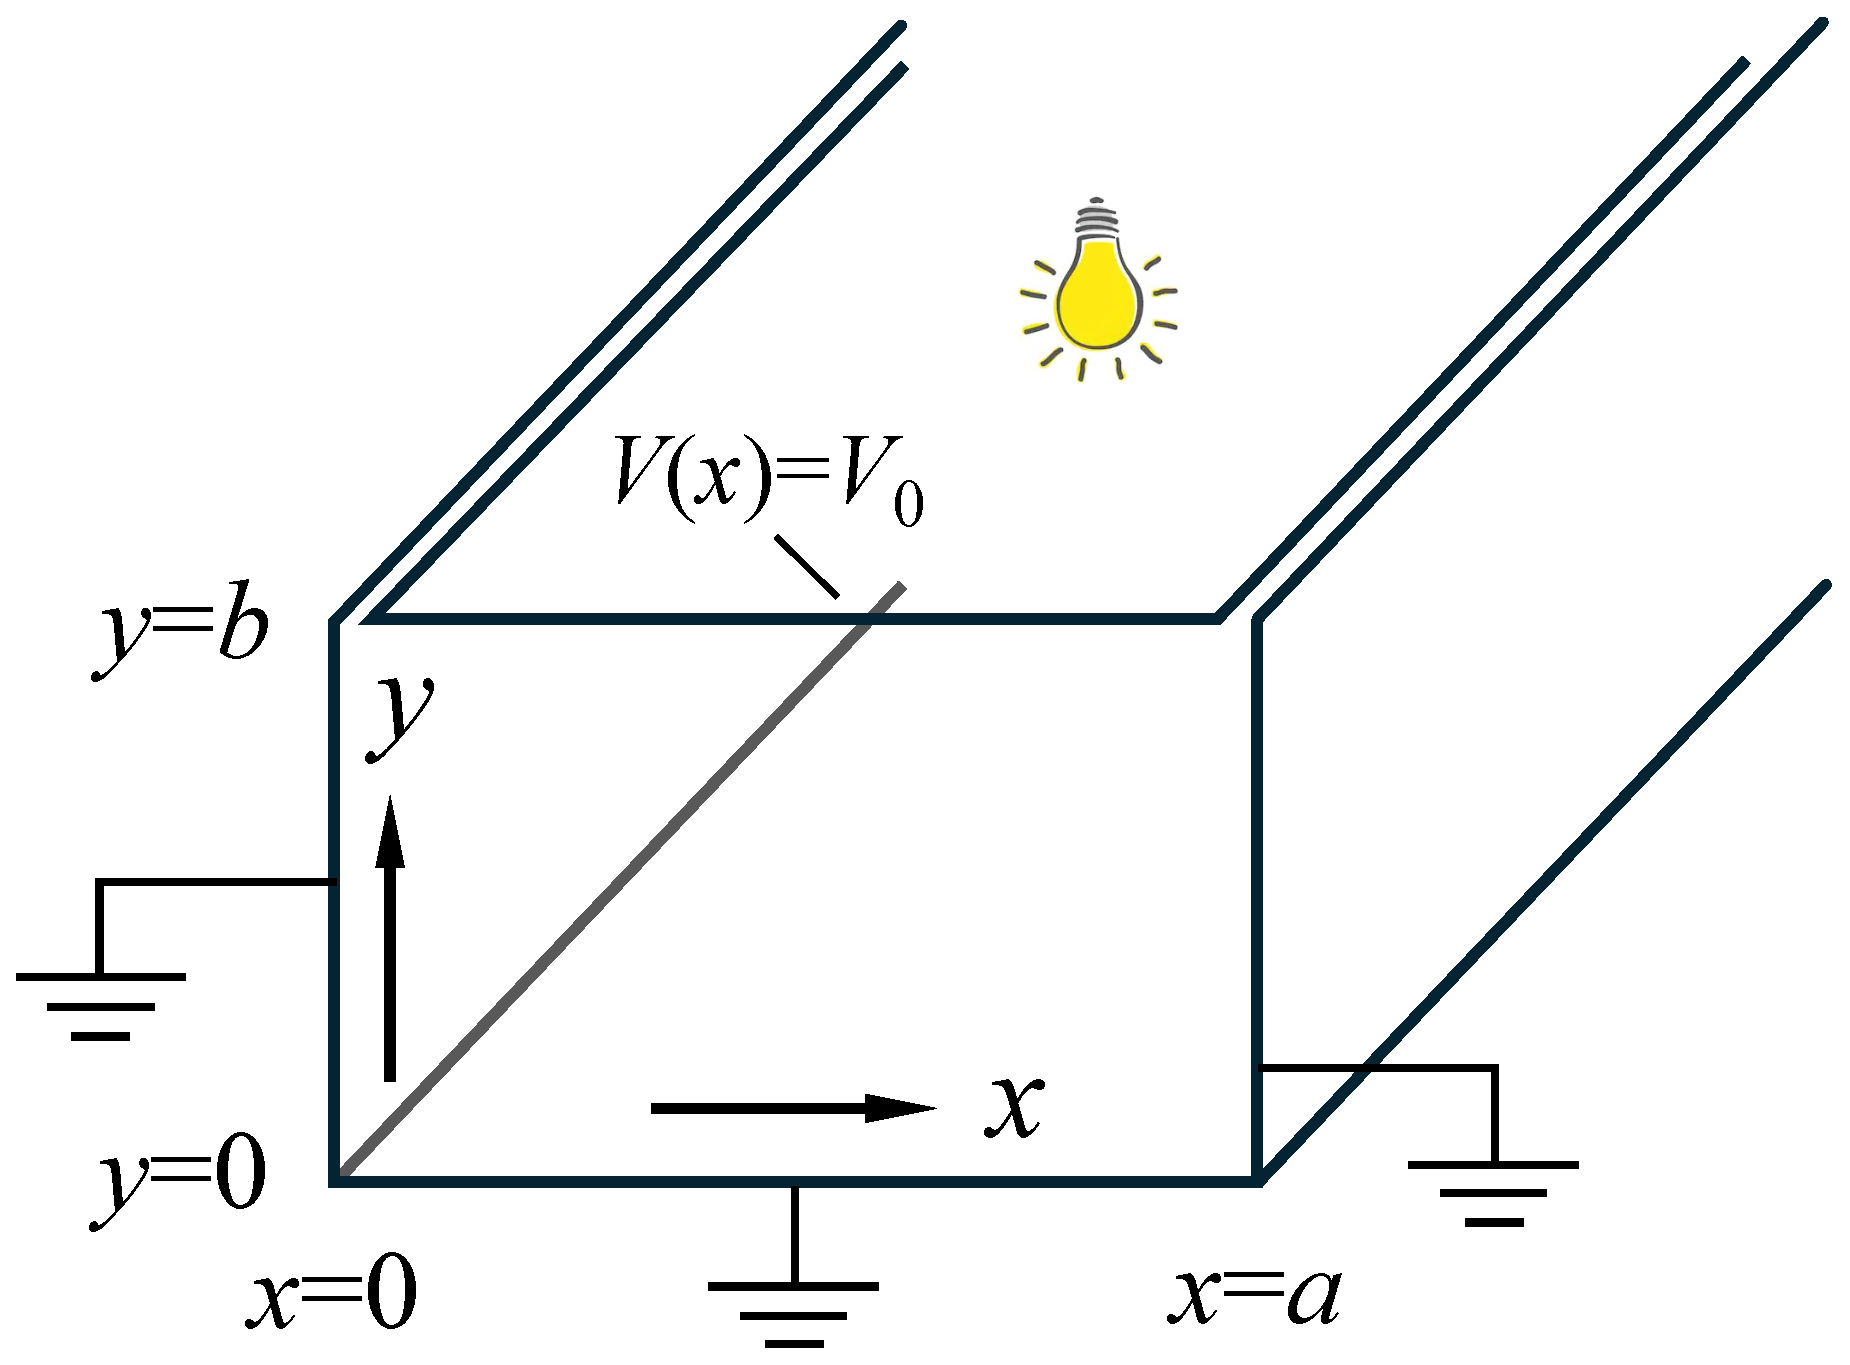
\includegraphics[width=0.5\linewidth]{./images/bulb_on_roof.eps}
    \caption{Sketch of the hospital corridor.}
    \label{fig:corridor}
\end{figure}

The next task is to calculate the potential in this corridor. This requires solving the Laplace equation.

\vspace{.3cm}  \hrule \vspace{.3cm}

Starting with Laplace's equation:
\[
    \nabla^{2}V = 0 
    \quad \to \quad 
    \frac{\partial^{2} V}{\partial x^{2}} + \frac{\partial^{2} V}{\partial y^{2}} + \cancelto{0}{\frac{\partial^{2} V}{\partial z^{2}}} = 0
\]
Here, we cancelled the $z$-direction term, as the corridor is straight and sufficiently long; by assumption, there is no variation of the electric potential in the $z$-direction. \\

To solve this $2^{\text{nd}}$-order partial differential equation, we employ the method of \textbf{separation of variables}. Using the relation solution: $V(x, y) = X(x) Y(y)$:
\[
    \frac{\partial^{2} V}{\partial x^{2}} + \frac{\partial^{2} V}{\partial y^{2}} 
    = 
    \frac{\partial^{2} X}{\partial x^{2}}y + \frac{\partial^{2} Y}{\partial y^{2}}x 
    = 0
\]
Divide both sides by $xy$:
\[
    \frac{1}{x} \frac{\partial^{2} X}{\partial x^{2}} + \frac{1}{y} \frac{\partial^{2} Y}{\partial y^{2}} = 0 
    \quad \Rightarrow \quad
    \frac{1}{x} \frac{\partial^{2} X}{\partial x^{2}} = -\frac{1}{y} \frac{\partial^{2} Y}{\partial y^{2}} = -k^{2}
\]
where $-k^2$ is a constant term, and it is commonly referred to as the \textit{separation constant}. By employing this method, the Laplace equation has been separated into two homogeneous ordinary differential equations (ODEs):
\[ 
    \frac{\partial^{2} X}{\partial x^{2}} + k^{2}x = 0 
    \quad \text{and} \quad 
    \frac{\partial^{2} Y}{\partial y^{2}} - k^{2}y = 0.
\]

To solve the $x$-dependent ODE: the characteristic equation $r^2-4k^2r = 0$, there exist two complex roots of $r$, hence, we conclude the general solution must be in the form 
\[
    x = A_{1}e^{jkx}+ A_{2}e^{-jkx},
\]
where $j$ denotes the imaginary unit, $A_1$ and $A_2$ are unknown constants subject to the boundary conditions. \\

To solve the $y$-dependent ODE: the characteristic equation $r^2+4k^2r = 0$, there exist two real roots of $r$, hence, we conclude the general solution must be in the form 
\[
    y = B_{1}e^{ky}+B_{2}e^{-ky}
\]
where $B_1$ and $B_2$ are unknown constants subject to the boundary conditions. \\

Therefore,
\[
    V(x, y)
    = X(x) Y(y) 
    = (A_{1}e^{jkx}+ A_{2}e^{-jkx}) (B_{1}e^{ky}+B_{2}e^{-ky}) 
\]
\hrule \vspace{.3cm}

Substitute 4 boundary conditions into $V(x, y)$:

\begin{enumerate}
    \item $V=0$ when $x=0$:
    \[ 
        0 = (A_{1}+A_{2})(B_{1}e^{ky}+B_{2}e^{-ky}) \quad \to \quad A_{1}=-A_{2}
    \]
    Therefore,
    \[
        V = A_{1}(e^{jkx}-e^{-jkx})(B_{1}e^{ky}+B_{2}e^{-ky})
    \]
    
    \item $V=0$ when $y=0$:
    \[
        0 = A_{1}(e^{jkx}-e^{-jkx})(B_{1}+B_{2}) \quad \to \quad 
        B_{1} = -B_{2} 
    \]
    Therefore,
    \[ 
        V = A_{1}B_{1}(e^{jkx}-e^{-jkx})(e^{ky}-e^{-ky})
    \]
    
   \item $V=0$ when $x=a$:
   \begin{align*} 
        0 
        &= A_{1}B_{1} \underbrace{(e^{jkx}-e^{-jkx})}_{=2j \sin (kx)} \underbrace{(e^{ky}-e^{-ky})}_{=2\sinh(ky)}\\[.5em]
        &= 4j A_{1}B_{1} \ \sin(ka) \ \sinh(ky)
    \end{align*}
    
    In this case, since $\sinh(ky)\neq 0$, and if $A_1 = 0$ or $B_1 = 0$, the solution will be trivial, therefore, $A_1\neq 0$ and $B_1\neq 0$. The only term left $\sin(ka)$ is 0. Let $k=\frac{n\pi}{a}$, where $n=1, 2, 3, ...$, we have:
    \begin{align*} 
    V 
        &= \underbrace{4 j A_{1} B_{1}}_{=C} \ \sin \left(\frac{n\pi}{a} x \right) \ \sinh \left(\frac{n\pi}{a} y \right) \\
        &= C \ \sin \left(\frac{n\pi}{a} x \right) \ \sinh \left( \frac{n\pi}{a} y \right)\\
     &= \sum^{\infty}_{n=1} C_{n} \sin \left( \frac{n\pi}{a} x \right) \ \sinh \left( \frac{n\pi}{a} y \right)
    \end{align*}
    
    \item $V=V(x)$ when $y=b$:
        \[  
            V(x) = \sum^{\infty}_{n=1} C_{n} \sin\left(\frac{n\pi}{a} x \right) \ \sinh\left(\frac{n\pi}{a} b\right)
        \]
        Let 
        \[ 
            D_{n} = C_{n} \sinh\left(\frac{n\pi}{a} b \right)
        \]
    Therefore, we can obtain the Fourier series:
    \[
        V(x) = \sum^{\infty}_{n=1} D_{n} \sin\left( \frac{n\pi}{a} x \right) 
    \]
   For $V(x) = V_{0}$, expand $D_{n} $:
   \begin{align*}
    D_{n}
    & = \frac{2}{a} \int_{0}^{a} V_{0} \sin\left(\frac{n\pi}{a} x\right) \mathrm{d}x \\
    & = -\frac{2}{a} \bigg[ \frac{aV_{0}}{n\pi} \cos\left(\frac{n\pi}{a} x\right) \bigg]^{a}_{0}\\
    & = \frac{2V_{0}}{n\pi}(1-(-1)^{n})
    \end{align*}
    Note that: if $n$ takes an even number, $D_{n}=\frac{4V_{0}}{n\pi} $; $n$ can never take odd numbers.
\end{enumerate}
 \hrule \vspace{.3cm}
 
We can recover the expression for $C_{n}$, then find the expression for $V$:
\[
    V(x, y) = \sum^{\infty}_{n=1} \frac{2V_{0}}{n\pi \ \sinh(\frac{n\pi}{a} b)} \ \sin \left( \frac{n\pi}{a} x \right) \ \sinh \left( \frac{n\pi}{a} y \right) 
\]
As $n$ increases, we can obtain a Fourier series that tends to have a constant value. 

\begin{figure}[H]
    \centering
    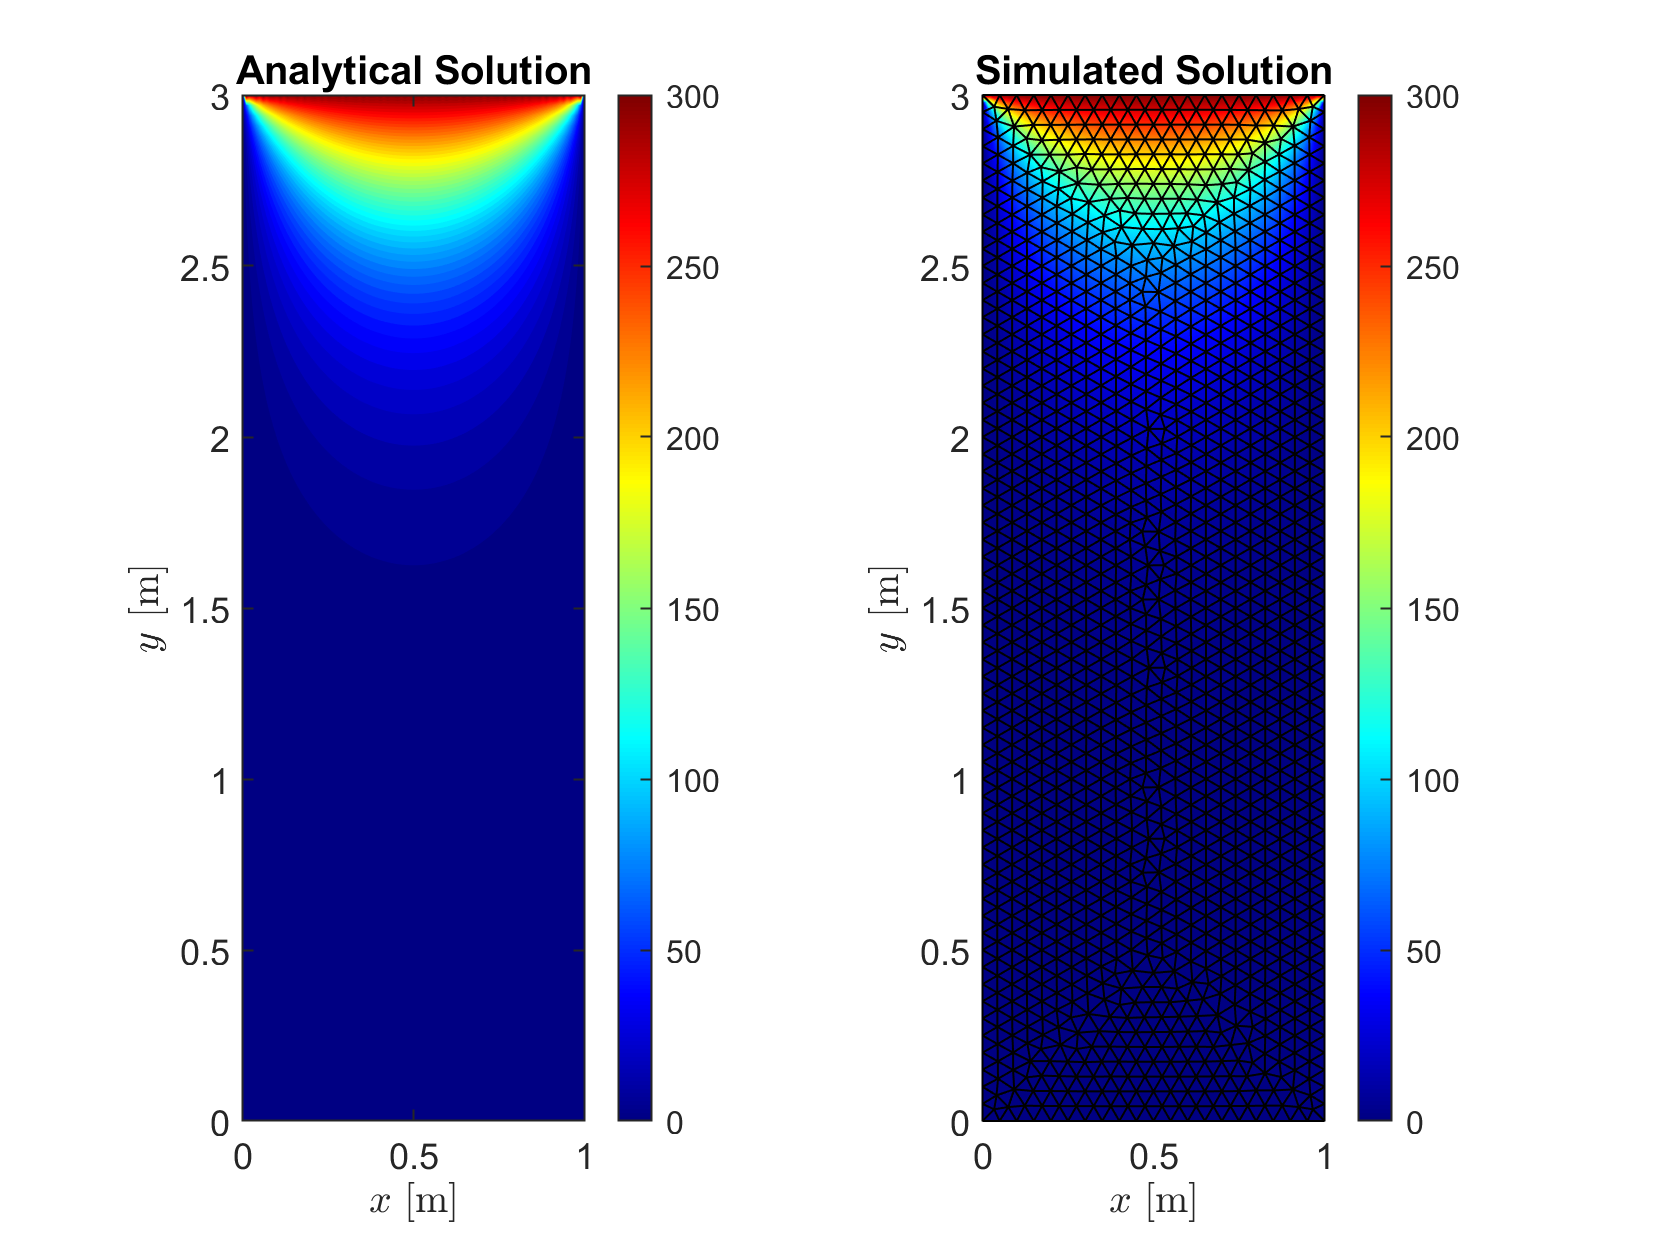
\includegraphics[width=0.9\linewidth]{./images/corridor_sol.png}
    \caption{Analytical (left) and numerical (finite element simulation) solution plot of the electric potential field $V(x, y)$ with $a=1$ m, $b=3$ m, $V_0=300$ V, and $n=81$.}
    \label{fig:corridor_sol}
\end{figure}
\end{mdframed}


\vfill
-----

Notes by \textbf{Binghuan Li}, last compiled on \today. This example is adopted from the lectures of Electronics and Electromagnetics 2 at the Department of Bioengineering, Imperial College London, delivered by Martin Holloway.  

\end{document}